%% LyX 2.0.3 created this file.  For more info, see http://www.lyx.org/.
%% Do not edit unless you really know what you are doing.
\documentclass[english]{aiaa-tc}
\usepackage[T1]{fontenc}
\usepackage[latin9]{inputenc}
\usepackage{array}
\usepackage{wrapfig}
\usepackage{units}
\usepackage{multirow}
\usepackage{amsmath}
\usepackage{amssymb}
\usepackage{mathdots}
\usepackage{graphicx}
\usepackage{esint}
\usepackage{nomencl}
% the following is useful when we have the old nomencl.sty package
\providecommand{\printnomenclature}{\printglossary}
\providecommand{\makenomenclature}{\makeglossary}
\makenomenclature

\makeatletter

%%%%%%%%%%%%%%%%%%%%%%%%%%%%%% LyX specific LaTeX commands.
%% Because html converters don't know tabularnewline
\providecommand{\tabularnewline}{\\}

%%%%%%%%%%%%%%%%%%%%%%%%%%%%%% User specified LaTeX commands.
\newcommand{\qed}{\hspace*{\fill}~$\square$}
\newcommand{\mqed}{\tag*{$\square$}}

% Added this to the preamble to deal with LyX's stupidity.
% That is, whenever you use a subfigure in LyX, LyX adds the lines
%---------------------
% \@ifundefined{showcaptionsetup}{}{%
% \PassOptionsToPackage{caption=false}{subfig}}
% \usepackage{subfig}
% \makeatother
% \usepackage[caption=false]{subfig}     % subfigures
%-----------------------
% Unfortunately this messes up whatever AIAA has done to adjust
% captions to suit its style. I have added the following to be used as
% part of a LyX template (which includes my AIAA LyX layout file) to
% fix this.

% This fixes the float captions
 % pass [caption=false] to prevent LyX from screwing up the captions
\usepackage[caption=false]{subfig} 

% This fixes the subfloat captions
% This introduces the capability to use a single parenthesis for subfloats.
\DeclareCaptionLabelSeparator{paren}{) }
% Set the font for subfloat captions
\captionsetup[subfloat]{ %
 % This makes the subcaptions bold.
font={footnotesize,bf}, %
 % This eliminates both parentheses around the subfloat label.
 labelformat=simple, %
 % This uses a right parenthisis as a separator.
 labelsep=paren % this came from the \DeclareCaptionLabelSeparator above
}

\@ifundefined{showcaptionsetup}{}{%
 \PassOptionsToPackage{caption=false}{subfig}}
\usepackage{subfig}
\makeatother

\usepackage{babel}
\begin{document}

\title{Multi-Disciplinary Cyber-Physical Optimization for Unmanned Aircraft
Systems}


\author{Justin M. Bradley and Meghan Clark}
\maketitle
\begin{abstract}
(Meghan)
\end{abstract}
\settowidth{\nomlabelwidth}{$P_{\rm{max}}^{s}$}
\printnomenclature{}


\section{Introduction (Justin)}

Modern systems require sensors, actuators, algorithms, and real-time
digital systems to coordinate their activities with a physical system
to achieve designated goals. Often each of these individual subsystems
are designed independently to meet performance objectives. Compositionality
and composability can suffer without co-design techniques that account
for limitations and strengths of each subsystem as well as the physical
system with which the system interacts. Additionally, as systems become
smaller, requiring less energy for actuation and sensing, computational
(cyber) resources begin to demand resources comparable to that of
the physical system.

Control systems engineers attempt to optimize physical system trajectories
by the proper application of force over time. Physics-based models
of system dynamics including saturation constraints and other nonlinearities
are used to design control laws that achieve designed trajectories
- most often in the continuous time domain. On the other hand, real-time
systems engineers, using discrete mathematical tools, optimize task
allocation and scheduling over processor, communication, and I/O resources
to guarantee performance deadlines for reliability and robustness.
Good design of the task schedule may provide enough slack so that
energy can be conserved through variable speed processors. Alternatively,
slack in the task schedule may allow for aperiodic and sporadic task
guarantees thereby providing event-driven capabilities or simply just
increased service of individual tasks.

For systems which must more carefully manage all their physical and
cyber resources together to achieve their objectives, globally-optimal
(minimum-energy, minimum-time, maximum-information) performance can
only be achieved by identifying and exploiting coupling between cyber
and physical resources during the design process. Cyber resources
provide the means for guidance, navigation, and control of the physical
system, as well as the estimation of states, communication, and processing
of information. The physical system, in turn, provides the ability
to acquire information, survey an area, or take important measurements.

We have been conducting research to try and accomplish such optimal
cyber-physical design. In~\cite{bradley2012multidisciplinary} we
developed a multidisciplinary approach for optimizing over both cyber
and physical resources and including mission goals and objectives.
Using metrics encompassing physical system energy, time, surveillance
information, and cyber utilization we showed that we can more appropriately
balance overall system performance. We also used pareto front analysis
to examine some of the coupling between cyber and physical resource
use.

In this report we take this research a step further by trying to experimentally
validate this technique. To this end we have adopted TableSat~\cite{vess2005system},
a one-degree of freedom rotating platform emulating a small satellite
to demonstrate this method of design. TableSat, shown in Figure~\ref{fig:TableSat},
uses computer fan actuators, rate gyros, and accelerometers controlled
by an onboard Gumstix computing platform to control it's rotation.
\begin{figure}
\begin{centering}
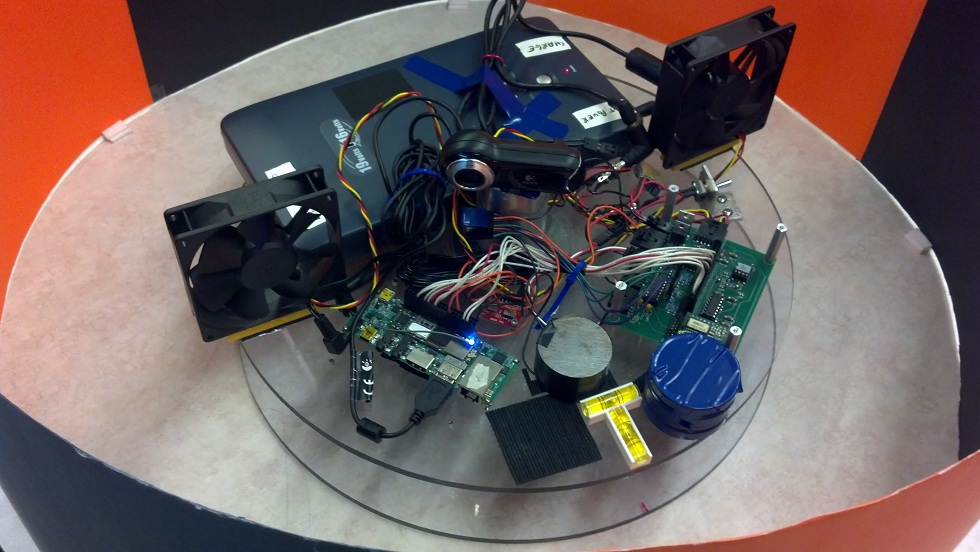
\includegraphics{pics/tablesat}
\par\end{centering}

\begin{centering}
\caption{TableSat\label{fig:TableSat}}

\par\end{centering}

\end{figure}


This paper presents a new multi-disciplinary optimization~\cite{andersson2000survey}
direction for which the models being integrated optimize energy consumption
over both physical effectors and computational (cyber) resources.
The cost function to be optimized includes weighted terms representing
energy used by physical actuators and energy used by a multi-core
or variable-speed processing architecture. This paper presents a case
study and appropriate UAS mission aimed at assessing the potential
performance improvements possible with co-optimization of cyber and
physical resources over energy use, time, and mission accomplishment.
A mission-appropriate analytical cost function is developed to provide
a minimal-cost trajectory over the mission. We simplify the cost function
by allowing design variables to remain static throughout the mission,
consistent with a steady flight scenario, thereby reducing the complexity
of the cost function and optimization process. We then examine Pareto
fronts for combinations of cost function objectives to demonstrate
the important tradeoffs between physical and cyber resources and to
give insight into the interdependence between them. We use a numerical
solver to find physical-subsystem optimal, cyber-subsystem optimal,
and holistic system optimal solutions and compare them with solutions
selected from Pareto front analysis. We demonstrate that only via
a total cyber-physical system (CPS) optimization can one achieve efficiency
throughout the total system.

For our case study, we adopt a solar-supplemented powered-glider small
UAS currently flown by a University of Michigan student team (SolarBubbles)
for which steady flight performance parameters are available. The
small UAS payload is a downward-facing video camera that can provide
frames at a variable rate. The simulated avionics allows direct regulation
of computational power requirements (energy use) in a manner that
trades energy use with camera data acquisition bandwidth. A one-dimensional
pipeline inspection case study is investigated, focusing attention
on physical and computational energy use tradeoffs without complexity
in the actual path through three-dimensional space.


\section{Related Work (Justin)}


\section{Cost Functions (Justin)}

We seek optimization over both physical and cyber characteristics
of the UAS in order to more holistically optimize system performance
for a designated mission. This means developing cost terms for task
performance and energy required for cyber activities as well as for
control actuation effort and propulsion. Moreover, we naturally want
to maximize efficiency of our designated mission which will include
goals for both the physical and cyber components of the UAS. These
mission-dependent goals may include maximizing coverage area or amount
of information acquired for a given area, along with collection, processing
and transmission of data. 

In this work we develop cost terms representing both mission goals
and efficiency for a UAS whose mission is surveillance of a straight
section of pipeline with a small, lightweight downward facing gimballed
camera. Because of this we focus on movement in one dimension only
and assume flight dynamics are governed by steady flight assumptions. 

Our objective for the physical system will be to determine the optimal
velocity (air speed in one dimension) of the UAS for the mission.
Owing to the assumptions of the mission and steady flight we rely
on a gimbal to consistently adjust the camera to point directly toward
the ground (optical axis perpendicular to ground plane) which compensates
for changes in pitch of the aircraft needed to accommodate various
velocities of flight. 

We model a single real-time task to accomplish the primary goals of
the mission related to pipeline surveillance. This task performs image
acquisition, processing, and communication/storage of image. Our design
objective for the cyber system will be to determine the optimal execution
rate of this task. While there are other system-critical tasks on
the cyber system including the control task, we assume these require
a fixed amount of resources. We instead focus on optimizing over the
remaining non-critical bandwidth available in the cyber system.

We divide the cost terms into physical and cyber goals for clarity,
and to emphasize the assimilation of each into a system-wide cost
function. ``Physical'' in the context of a UAS includes items related
to flight, for example, the airframe, propulsion system, and control
surfaces. ``Cyber'' relates to items required for data processing,
communication, image collection, computation of control inputs, etc.
In this work we endeavor to focus clearly on the idea of combining
physical and cyber cost terms into a holistic cyber-physical system
cost function.


\subsection{Physical System Terms}

Small UAS often have very modest energy reserves, most often consisting
of small battery packs, or a small fuel tank. In non-energy-harvesting
applications under normal conditions such energy supplies can provide
between thirty minutes to multiple hours of flight time. These flight
times can be reduced when cyber-intensive activities such as image
processing and communication are involved. Minimizing energy consumption
during steady flight is an important consideration in the design and
control of the UAS.


\subsubsection{Physical System Energy}

In most aircraft applications, propulsion will consume the majority
of the energy required for flight, surpassing actuation effort required
by control surfaces. For simplicity, in this work we assume propulsion
is the only drain on energy supplies by the physical system and we
model steady flight in which power used by control surface servos
would be constant or near-constant. We therefore seek to minimize
energy of the physical system over the entire mission\nomenclature{$E$}{Energy for the physical system}
\begin{equation}
E=\int P\left(v\left(t\right)\right)dt\label{eq:E}
\end{equation}
where $P\left(v\left(t\right)\right)$ is a traditional model for
power as a function of velocity~\cite{mcclamroch2011steady}\nomenclature{$P(v)$}{Power as a function of velocity}
\begin{equation}
P\left(v\right)=\frac{1}{2}C_{D_{0}}\rho v\left(t\right)_{air}^{3}+\frac{2KW^{2}}{\rho v\left(t\right)_{air}S}.\label{eq:power}
\end{equation}
\nomenclature{$K$}{Aerodynamic parameter}\nomenclature{$W$}{Weight}\nomenclature{$\rho$}{Air density}\nomenclature{$S$}{Wing surface area}\nomenclature{$C_{D_0}$}{Zero-lift drag coefficient}\begin{wrapfigure}{o}{0.5\columnwidth}%
\begin{centering}
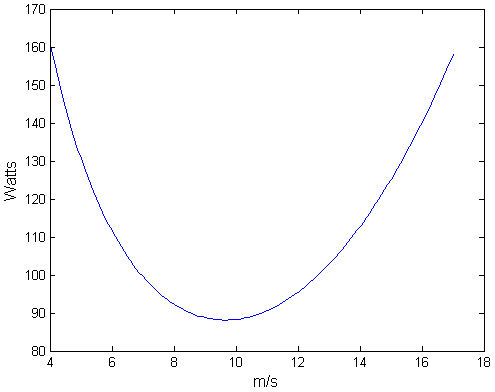
\includegraphics{pics/power_curve}
\par\end{centering}

\caption{Power Curve for SolarBubbles UAS\label{fig:Power-Curve}}
\end{wrapfigure}%
In steady level flight, power of the aircraft, and therefore velocity,
is manipulated by a throttle setting that maps nonlinearly to power
as
\begin{equation}
P=\eta\delta_{t}\left(\frac{\rho}{\rho^{s}}\right)^{m}P_{{\rm max}}^{s}
\end{equation}
where \nomenclature{$P_{\rm{max}}^{s}$}{Maximum power of the engine/motor at sea level}$P_{{\rm max}}^{s}$
is the maximum power of the engine/motor at sea level, $m>0$ is a
characteristic of the engine/motor, \nomenclature{$\eta$}{Propeller efficiency factor}$0\le\eta\le1$
is a propeller efficiency factor, \nomenclature{$\rho^s$}{Air density at sea level}$\rho^{s}$
is the air density at sea level, and \nomenclature{$\delta_t$}{Throttle setting}$0\le\delta_{t}\le1$
is the throttle setting. The power curve for our UAS (described in
Section~\ref{sub:Aircraft_description}) can be seen in Figure~\ref{fig:Power-Curve}.


\subsubsection{Time}

In addition to minimizing energy, ideally we would like to efficiently
accomplish our mission by minimizing the time required to complete
it. Such time-minimal optimization cost terms appear frequently and
are simply given by \nomenclature{$T$}{Total time required to complete mission}
\begin{equation}
T=\int dt.
\end{equation}



\subsubsection{Cost Function for Physical System}

These two competing objectives, $E_{p}$ and $T$, comprise the cost
function for the overall physical system 
\begin{equation}
J_{p}\left(v\left(t\right)\right)=\beta_{p1}\int P\left(v\left(t\right)\right)dt+\beta_{p2}\int dt\label{eq:J_p}
\end{equation}
\nomenclature{$J_p$}{Cost function for physical system}where $\beta_{p1},\,\beta_{p2}$
are weighting terms. Optimizing $J_{p}$ alone is what a traditional
trajectory or path planner would do if no costs are attributed to
the cyber system. While some UAS researchers have added tracking information,
target acquisition, and other mission objectives to their control
and optimization algorithms~\cite{zhan2005centralized,sinha2005autonomous},
to our knowledge this has historically been done from the physical
perspective without attempting to optimize over cyber system performance
and requirements.


\subsection{Cyber System Terms}

In a modern fully-autonomous UAS the cyber system becomes the gateway
for virtually all aspects of the system. Control actuation inputs,
data collection, communication, throttle setting, path and mission
planning are potentially all being done simultaneously on-board. While
real-time system researchers have advanced scheduling techniques for
prioritizing each of these critical tasks, the correlation between
physical performance, mission objectives, and computational efficiency
has remained largely unexplored.

In many cyber-physical systems (CPS)\nomenclature{CPS}{Cyber-Physical System}
task execution rates are selected \emph{a priori} based on requirements
of the system. For example, the sampling rate of the control task
may be selected based on digital control analysis. While it is unreasonable
to interfere with such high priority tasks, lower priority tasks may
still have some flexibility in task execution rate allowing us to
optimize over mission and cyber parameters without interfering with
mission critical tasks.

In our previous work we explored the tradeoff of mission critical
task execution rates and physical performance~\cite{bradley2011computational,bradley2012toward}.
For this work we assume that hard real-time feedback control tasks
are appropriately executed while we focus on the rest of the available
cyber resources for soft real-time tasks. More specifically, we assume
that we cannot only conserve energy by optimally selecting execution
rates of lower priority tasks, but we can also increase mission effectiveness
by developing costs that relate task execution rates to mission efficiency.


\subsubsection{Cyber Utilization}

We assume that at least part of the cyber utilization is fixed based
on selected and scheduled rates of mission critical tasks, and instead
focus on maximizing use of the remaining resources. To that end, we
assume a single task, \nomenclature{$\tau$}{Real-time system task achieving important mission goal}$\tau$,
achieves the important mission goal of capturing and processing an
image of the pipeline. The task runs at execution rate \nomenclature{$r_{\tau}$}{Task execution rate in Hz of task $\tau$}$\unit[r_{\tau}\left(k\right)]{Hz}$
and has a maximum execution rate of $\unit[r_{\tau,max}]{Hz}$ stemming
from restrictions based on available cyber resources. We introduce
the cyber utilization term\nomenclature{$U_\tau$}{Cyber utilization cost term}
\begin{equation}
U_{\tau}=\sum_{k}\frac{r_{\tau}\left(k\right)}{r_{\tau,max}}.\label{eq:U_tau}
\end{equation}
We note that $r_{\tau}\left(k\right)$ is the rate of execution of
task $\tau$ at discrete intervals $k$ and that the rate of execution
cannot change during a particular execution cycle of that task. We
assume that cyber utilization is proportional to energy consumed by
the cyber system, and as a result, minimizing it is the cyber equivalent
to the energy minimization term of the physical system in Equation~\eqref{eq:E}.


\subsubsection{Mission Information}

We seek to relate mission efficiency to cyber and physical parameters.
For our specified mission, we assume that detailed imagery of the
pipeline is critical for detecting aberrations and problems. Therefore,
we create a cost term based on overlap between successive images where
increasing overlap is rewarded. Acquiring multiple images of the same
ground points has the advantage of providing additional viewpoints
and redundant data, and may allow for super-resolved imagery thereby
increasing our ability to detect pipeline anomalies~\cite{ready2006kalmanfilter}.
From an information theory perspective we view information cost as
entropy for which an exponential distribution indicates the quantity
of unknown information associated with points on the overflown region
(or pipeline). In this sense, minimizing the entropy has the effect
of maximizing the total information acquired. This term has the effect
of requiring a combination of slow aircraft speed and/or increased
task frequency and depends on both velocity of the aircraft, $v\left(t\right)$,
and rate of image acquisition and processing $r_{\tau}\left(k\right)$\nomenclature{$H$}{Entropy cost}
\begin{equation}
H=\int e^{-\alpha\Omega\left(v\left(t\right),r_{\tau}\left(k\right)\right)}dt.\label{eq:H}
\end{equation}
\begin{wrapfigure}[17]{i}{0.49\textwidth}%
\vspace{-7pt}


\begin{centering}
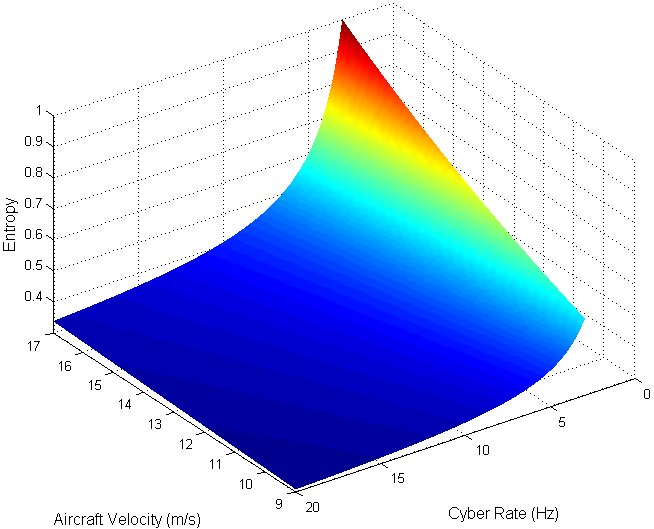
\includegraphics{pics/plot_H}
\par\end{centering}

\caption{Entropy Cost $H$\label{fig:Entropy-Cost}}


\end{wrapfigure}%
We let \nomenclature{$\alpha$}{Tuning parameter in entropy cost}$\alpha$
be a tuning parameter, and 
\begin{equation}
\Omega\left(v\left(t\right),r_{\tau}\left(k\right)\right)=\frac{1}{A}\left(A-w\int_{t-T_{\tau}\left(k\right)}^{t}v\left(\gamma\right)d\gamma\right)
\end{equation}
where \nomenclature{$A$}{Area of an image}$A$ is the total area
of an image, \nomenclature{$w$}{Width of an image}$w$ is the width
of an image, and \nomenclature{$T_\tau$}{Period of task $\tau$}$T_{\tau}\left(k\right)=\unitfrac{1}{r_{\tau}\left(k\right)}$
is the period of task $\tau$. For simplicity, we assume that the
aircraft flies at approximately the same height above ground for the
mission, and therefore $A$ and $w$ remain constant. In Figure~\ref{fig:Entropy-Cost}
we show a plot of $H$ to demonstrate how the entropy changes with
both cyber rate $\left(r_{\tau}\right)$ and velocity $\left(v\right)$.
The dependence of entropy on cyber rate falls off as a steep exponential,
and falls off more gradually with aircraft velocity. This means we
expect our Pareto front analysis in Section~\ref{sub:Pareto-Fronts}
to indicate lower entropy by increasing cyber rate than by going slower.


\subsubsection{Cost Function for Cyber System}

The expressions in Equations~\eqref{eq:U_tau} and~\eqref{eq:H}
comprise the cost function for the cyber system
\begin{equation}
J_{c}\left(v\left(t\right),r_{\tau}\left(k\right)\right)=\beta_{c1}\sum_{k}\frac{r_{\tau}\left(k\right)}{r_{\tau,max}}+\beta_{c2}\int e^{-\alpha\Omega\left(v\left(t\right),r_{\tau}\left(k\right)\right)}dts\label{eq:J_c}
\end{equation}
where we have weighting terms $\beta_{c1}$, and $\beta_{c2}$. Such
a cost function might be used if we were only interested in trading
cyber resource utilization cost against reward from accomplishing
mission objectives, which in the pipeline inspection case study maps
to minimizing entropy (unknown information) that could be obtained
through overlapping image data acquisition and processing.


\subsection{CPS Cost Function}

We combine $J_{p}$ and $J_{c}$ to obtain a holistic CPS cost function
\begin{equation}
J\left(v\left(t\right),r_{\tau}\left(k\right)\right)=\beta_{p1}\int P\left(v\left(t\right)\right)dt+\beta_{p2}\int dt+\beta_{c1}\sum_{k}\frac{r_{\tau}\left(k\right)}{r_{\tau,max}}+\beta_{c2}\int e^{-\alpha\Omega\left(v\left(t\right),r_{\tau}\left(k\right)\right)}dt\label{eq:J}
\end{equation}


In Section~\ref{sec:Results} we will use appropriate weighting to
compare physical-only optimization, cyber-only optimization, and total
system optimization to demonstrate how increased efficiency and conservation
of energy can be achieved by including both physical and cyber objectives.


\subsection{Simplified Cost Function}


\subsubsection{Analytical Solution and Feasibility}


\section{TableSat Details (Meghan)}

Our objective is to survey a straight segment of pipeline by flying
a small, high aspect ratio UAS with a downward facing gimballed camera
directly overhead. We have created a simulation in MATLAB to compare
various solutions to the optimization problem posed. We first mention
the assumptions we've made to simplify the problem and demonstrate
why an analytical solution is not possible. We then describe the numerical
methods chosen to solve our optimization problem, and discuss the
models we have adopted. 


\subsection{Assumptions}


\subsection{Experimental Models and Setup}


\subsubsection{TableSat}

bar


\subsubsection{Camera}

foo


\subsubsection{Gumstix}

foo


\subsubsection{Cyclic Executive}


\section{Analytical Results (Justin)\label{sec:Results}}

We investigated the impact and tradeoffs between objectives from both
the cyber and physical systems with the goal of minimizing energy
use and time while maximizing information (minimizing entropy). Our
goal is to show that simultaneous consideration of cyber and physical
cost terms can yield more capable missions than what would be possible
from designing these two parts of the CPS individually. We first examine
and analyze Pareto fronts of the cost function in Equation~\eqref{eq:J_new}
to gain insight into the tradeoffs from competing objectives. We select
candidate points along the Pareto front of several plots and use the
corresponding $v$ and $r_{\tau}$ to compute associated costs of
the mission. We then select weights $\beta_{p1},\,\beta_{p2},\,\beta_{c1}$,
and $\beta_{c2}$, optimize the CPS cost function in Equation~\eqref{eq:J_new}
and compare results with solution points selected from the Pareto
fronts.


\subsection{Numerical method}


\subsection{Pareto Fronts\label{sub:Pareto-Fronts}}

Pareto front examination and analysis gives insight into the tradeoffs
between competing objectives. Pareto front plots of $J_{p}$ (Equation~\eqref{eq:J_p})
and $J_{c}$ (Equation~\eqref{eq:J_c}) can be seen in Figure~\ref{fig:Pareto-Front-J_p-and-J_c}
where the black (darker) data points represent the Pareto front.
\begin{figure}
\noindent \begin{centering}
\subfloat[Pareto Front for $J_{p}$\label{fig:Pareto-Front-for-J_p} ]{\noindent \begin{centering}
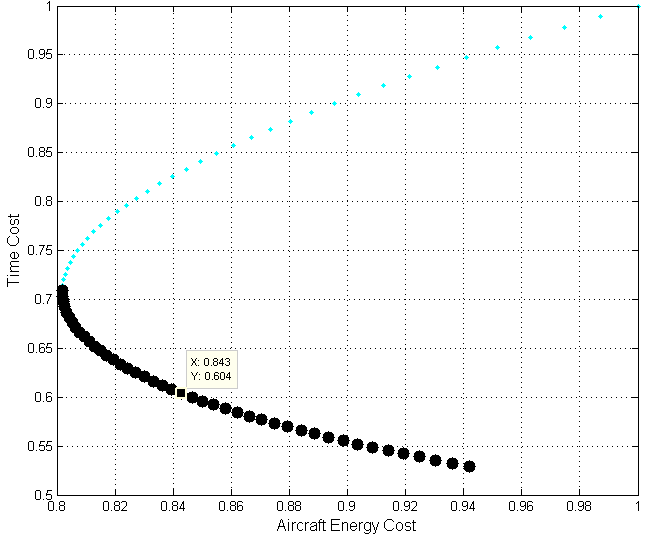
\includegraphics[width=0.45\textwidth]{pics/pareto_J_p}
\par\end{centering}

}\subfloat[Pareto Front for $J_{c}$\label{fig:Pareto-Front-for-J_c}]{\noindent \begin{centering}
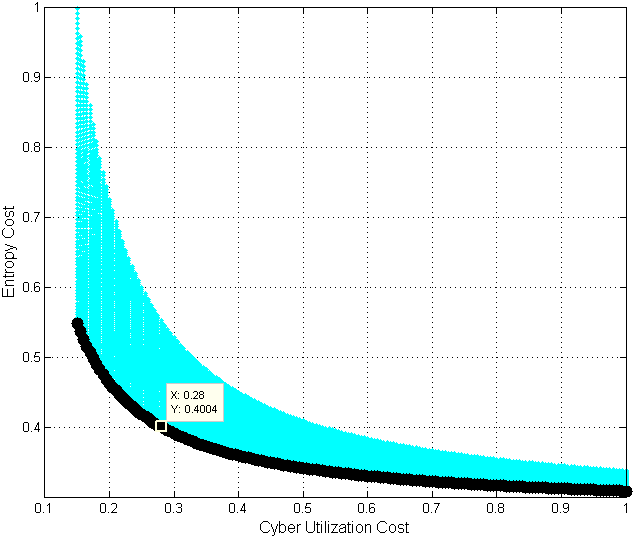
\includegraphics[width=0.45\textwidth]{pics/pareto_J_c}
\par\end{centering}

}
\par\end{centering}

\caption{Pareto Front for $J_{p}$ and $J_{c}$\label{fig:Pareto-Front-J_p-and-J_c}}
\end{figure}
 

These curves show how the objectives for the physical and cyber system,
individually, trade off their respective costs. The plots in Figure~\ref{fig:Pareto-Front-J_p-and-J_c}
follow their respective governing dynamical equations to produce the
curves shown. For Figure~\ref{fig:Pareto-Front-for-J_p} the plot
is dominated by the power curve indicating we could expend similar
amounts of energy, accomplishing our mission in very different lengths
of time. Clearly to achieve our minimum time objective, the front
side of the power curve is more optimal as indicated by the Pareto
front. Because our entropy cost is a function of both $v$ and $r_{\tau}$
we have multiple points corresponding to a single cyber rate $r_{\tau}$.
As a result, the velocities resulting in a higher entropy cost are
dominated by those producing lower entropy.

If we choose a solution along the Pareto front we will optimize for
either the physical or cyber portion of the system. Using these plots,
we select the velocity corresponding with the data point highlighted
in Figure~\ref{fig:Pareto-Front-for-J_p}, $v=\unit[14.9]{\unitfrac{m}{s}}$
. From the Pareto front for $J_{c}$ we choose the cyber rate corresponding
with the data point highlighted in Figure~\ref{fig:Pareto-Front-for-J_c},
or $r_{\tau}=\unit[5.6]{Hz}$. 
\begin{table}
\caption{Costs For $v=\unit[14.9]{\unitfrac{m}{s}}$ and $r_{\tau}=\unit[5.6]{Hz}$\label{tab:Costs-individual}}


\noindent \centering{}%
\begin{tabular}{|c|c|c|c|c|}
\hline 
Parameters & $E$ & $T$ & $U_{\tau}$ & $H$\tabularnewline
\hline 
\hline 
$v=\unit[14.9]{\unitfrac{m}{s}},\, r_{\tau}=\unit[5.6]{Hz}$ & $\unit[16626.2]{J}$ & $\unit[134.2]{s}$ & $0.28$ & $66.7$\tabularnewline
\hline 
\end{tabular}
\end{table}
In Table~\ref{tab:Costs-individual} we show the costs associated
with a mission using these parameters.

We can gain more insight into the tradeoffs of the entire cost function
by also examining the tradeoffs between the CPS as a whole. We show
these Pareto fronts in Figure~\ref{fig:pareto_J} where in each subfigure
we examine the tradeoff between three of the four objectives.
\begin{figure}
\noindent \begin{centering}
\subfloat[Pareto Front for $E,\, U_{\tau}$, and $H$\label{fig:pareto_E_U_H}]{\noindent \begin{centering}
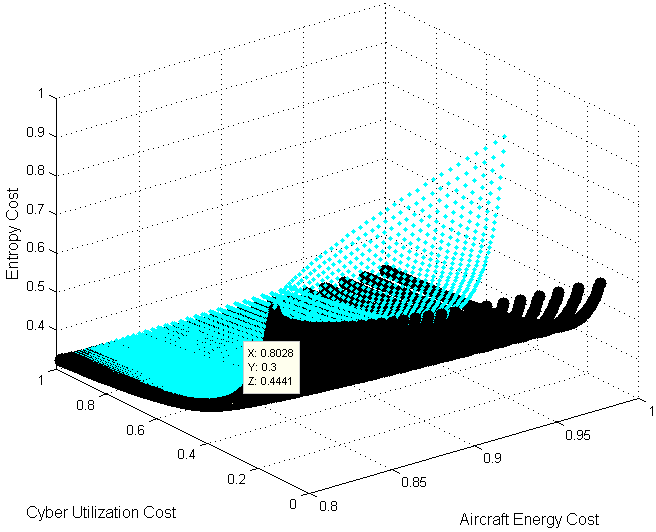
\includegraphics[width=0.45\textwidth]{pics/pareto_J_ac_cu_i}
\par\end{centering}

}\subfloat[Pareto Front for $E,\, T$, and $U_{\tau}$\label{fig:pareto_E_T_U} ]{\noindent \begin{centering}
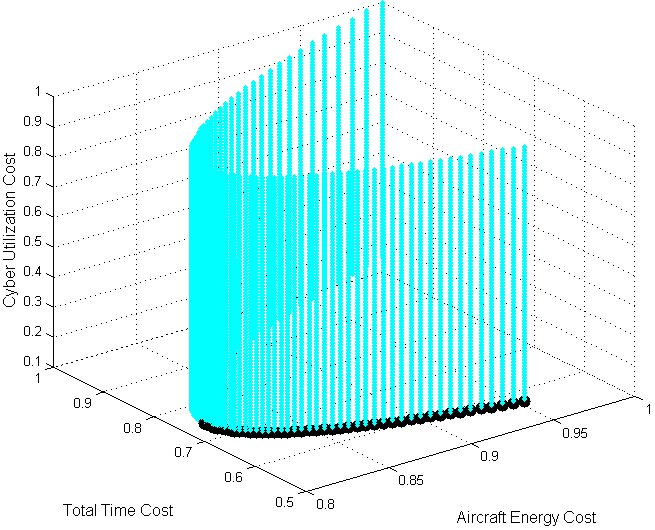
\includegraphics[width=0.45\textwidth]{pics/pareto_J_ac_t_cu}
\par\end{centering}

}
\par\end{centering}

\noindent \begin{centering}
\subfloat[Pareto Front for $H,\, T$, and $U_{\tau}$\label{fig:pareto_H_T_U}]{\noindent \begin{centering}
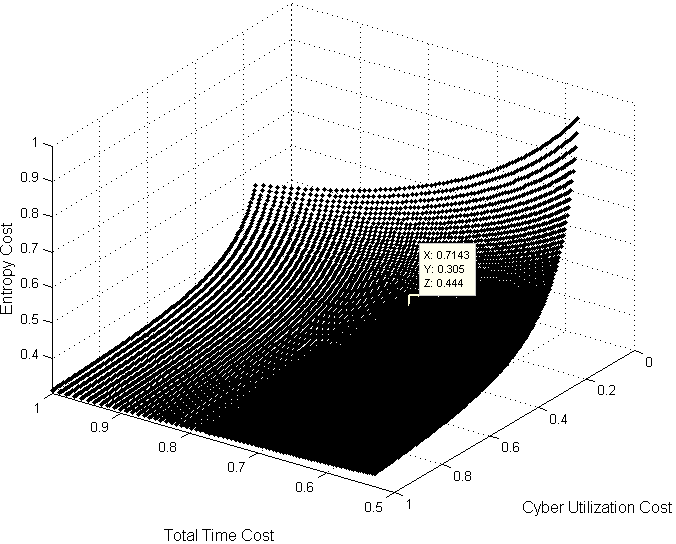
\includegraphics[width=0.45\textwidth]{pics/pareto_J_i_t_cu}
\par\end{centering}

}\subfloat[Pareto Front for $H,\, T$, and $E$\label{fig:pareto_H_T_E}]{\noindent \begin{centering}
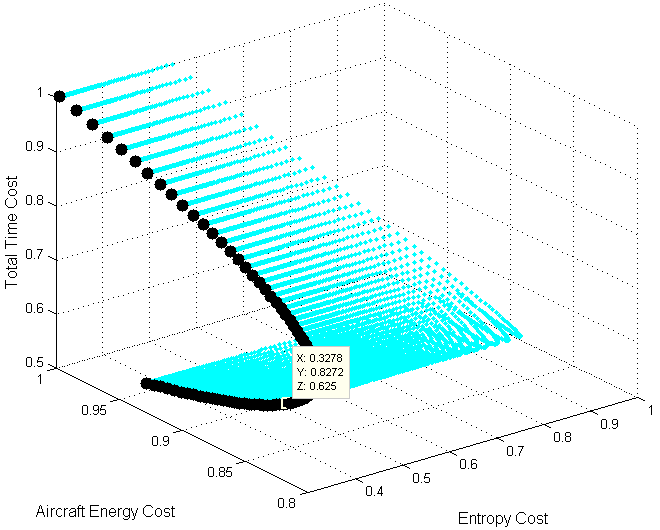
\includegraphics[width=0.45\textwidth]{pics/pareto_J_i_t_ac}
\par\end{centering}

}
\par\end{centering}

\caption{Pareto Fronts for $J$\label{fig:pareto_J}}
\end{figure}
 In Figure~\ref{fig:pareto_E_U_H} we again observe the presence
of the power curve governing the relationship between aircraft energy
$\left(E\right)$ and the other objectives. The curve folds over onto
itself and we choose the point indicated in that plot which is in
the crease of the function while also balancing cyber utilization
$\left(U_{\tau}\right)$ and entropy $\left(H\right)$ costs.

In Figure~\ref{fig:pareto_E_T_U} no new insight or information is
gained since the Aircraft Energy cost and Total Time cost $\left(T\right)$
are independent of Cyber Utilization cost. Additionally, we note the
similarity of this plot with the Pareto front for $J_{p}$ in Figure~\ref{fig:Pareto-Front-for-J_p}.
In the Pareto front plot in Figure~\ref{fig:pareto_H_T_U} there
are no dominated points making the entire surface a Pareto front.
We select the solution point indicated on this Pareto front based
on intuition.

Figure~\ref{fig:pareto_H_T_E} shows the tradeoffs between entropy,
aircraft energy, and total time costs. In this Pareto front we call
attention to the normal tradeoff between total time and aircraft energy
costs, but more interestingly the tradeoff with entropy cost. This
shows the coupling between cyber and physical cost terms and gives
insight into how they compete in the total cost. We follow our previous
reasoning in choosing a point that compromises total time and aircraft
energy but augmented by an attempt to minimize entropy as well.

We list the velocities, cyber rates, and corresponding costs for each
of these three selected points in Table~\ref{tab:params_costs_pareto_3}.
\begin{table}
\caption{Parameters and Costs for Data Points Selected from Pareto Fronts\label{tab:params_costs_pareto_3}}


\noindent \centering{}%
\begin{tabular}{|c|c|c|c|c|}
\hline 
Parameters & $E$ & $T$ & $U_{\tau}$ & $H$\tabularnewline
\hline 
\hline 
$v=\unit[14.4]{\unitfrac{m}{s}},\, r_{\tau}=\unit[15.4]{Hz}$ & $\unit[16314.5]{J}$ & $\unit[138.9]{s}$ & $0.77$ & $45.2$\tabularnewline
\hline 
$v=\unit[12.4]{\unitfrac{m}{s}},\, r_{\tau}=\unit[6]{Hz}$ & $\unit[15833.3]{J}$ & $\unit[161.3]{s}$ & $0.30$ & $58.4$\tabularnewline
\hline 
$v=\unit[12.6]{\unitfrac{m}{s}},\, r_{\tau}=\unit[6.1]{Hz}$ & $\unit[15816.9]{J}$ & $\unit[158.7]{s}$ & $0.31$ & $58.4$\tabularnewline
\hline 
\end{tabular}
\end{table}
 


\subsection{Optimization over Total Cost Function $J\left(v,r_{\tau}\right)$}

In addition to examining Pareto fronts, using numerical methods, we
can solve $J\left(v,r_{\tau}\right)$ in Equation~\eqref{eq:J_new},
examine the resulting costs, and compare them with those found from
the Pareto front analysis. This requires we select the weights for
each cost term. Often there are auxiliary reasons for favoring one
cost term over another such as length of time since the last mission,
or a cloudy day with less direct sunshine resulting in a tighter energy
budget for our solar powered glider. Since we wish to investigate
the comparison of holistic CPS optimization with independent physical
and cyber system optimization we allow corresponding weights to go
to zero as indicated in the $5^{th}$ and $6^{th}$ rows of Table~\ref{tab:Comparison-of-All}.
In each case, however, in the absence of any compelling reasons to
favor one term over another we equalize all non-zero cost terms as
shown. We compare the previous results from our Pareto analysis with
our numerical solutions and show the individual costs, as well as
the scaled, and normalized total cost in Table~\ref{tab:Comparison-of-All}.
\begin{table}
\caption{Comparison of All Solutions\label{tab:Comparison-of-All}}


\noindent \centering{}%
\begin{tabular}{|c|c|c|c|c|c|c|c|}
\hline 
\multirow{2}{*}{Parameters} & \multirow{2}{*}{Solution Type} & \multirow{2}{*}{$E$} & \multirow{2}{*}{$T$} & \multirow{2}{*}{$U_{\tau}$} & \multirow{2}{*}{$H$} & \multirow{2}{*}{Total} & \% Worse than\tabularnewline
 &  &  &  &  &  &  & Lowest Cost Soln.\tabularnewline
\hline 
\hline 
$v=\unit[14.9]{\unitfrac{m}{s}}$ & \multirow{2}{*}{Pareto from Table~\ref{tab:Costs-individual}} & \multirow{2}{*}{$\unit[16626.2]{J}$} & \multirow{2}{*}{$\unit[134.2]{s}$} & \multirow{2}{*}{$0.28$} & \multirow{2}{*}{$66.7$} & \multirow{2}{*}{0.5587} & \multirow{2}{*}{$0.25\%$}\tabularnewline
$r_{\tau}=\unit[5.6]{Hz}$ &  &  &  &  &  &  & \tabularnewline
\hline 
$v=\unit[14.4]{\unitfrac{m}{s}}$ & \multirow{2}{*}{Pareto from Table~\ref{tab:params_costs_pareto_3}} & \multirow{2}{*}{$\unit[16314.5]{J}$} & \multirow{2}{*}{$\unit[138.9]{s}$} & \multirow{2}{*}{$0.77$} & \multirow{2}{*}{$45.2$} & \multirow{2}{*}{$0.6416$} & \multirow{2}{*}{$15.13\%$}\tabularnewline
$r_{\tau}=\unit[15.4]{Hz}$ &  &  &  &  &  &  & \tabularnewline
\hline 
$v=\unit[12.4]{\unitfrac{m}{s}}$ & \multirow{2}{*}{Pareto from Table~\ref{tab:params_costs_pareto_3}} & \multirow{2}{*}{$\unit[15833.3]{J}$} & \multirow{2}{*}{$\unit[161.3]{s}$} & \multirow{2}{*}{$0.30$} & \multirow{2}{*}{$58.4$} & \multirow{2}{*}{$0.5682$} & \multirow{2}{*}{$1.96\%$}\tabularnewline
$r_{\tau}=\unit[6]{Hz}$ &  &  &  &  &  &  & \tabularnewline
\hline 
$v=\unit[12.6]{\unitfrac{m}{s}}$ & \multirow{2}{*}{Pareto from Table~\ref{tab:params_costs_pareto_3}} & \multirow{2}{*}{$\unit[15816.9]{J}$} & \multirow{2}{*}{$\unit[158.7]{s}$} & \multirow{2}{*}{$0.31$} & \multirow{2}{*}{$58.4$} & \multirow{2}{*}{$0.5663$} & \multirow{2}{*}{$1.61\%$}\tabularnewline
$r_{\tau}=\unit[6.1]{Hz}$ &  &  &  &  &  &  & \tabularnewline
\hline 
$v=\unit[15.2]{\unitfrac{m}{s}}$ & $J$ with $\beta_{p1}=\beta_{p2}=0.5$ & \multirow{2}{*}{$\unit[16844.1]{J}$} & \multirow{2}{*}{$\unit[131.6]{s}$} & \multirow{2}{*}{$0.90$} & \multirow{2}{*}{$44.3$} & \multirow{2}{*}{$0.6708$} & \multirow{2}{*}{$20.37\%$}\tabularnewline
$r_{\tau}=\unit[18]{Hz}$ & $\beta_{c1}=\beta_{c2}=0.0$ &  &  &  &  &  & \tabularnewline
\hline 
$v=\unit[9.0]{\unitfrac{m}{s}}$ & $J$ with $\beta_{p1}=\beta_{p2}=0.0$ & \multirow{2}{*}{$\unit[19722.8]{J}$} & \multirow{2}{*}{$\unit[222.2]{s}$} & \multirow{2}{*}{$0.22$} & \multirow{2}{*}{$58.7$} & \multirow{2}{*}{$0.6654$} & \multirow{2}{*}{$19.40\%$}\tabularnewline
$r_{\tau}=\unit[4.3]{Hz}$ & $\beta_{c1}=\beta_{c2}=0.5$ &  &  &  &  &  & \tabularnewline
\hline 
$v=\unit[14.2]{\unitfrac{m}{s}}$ & $J$ with $\beta_{p1}=\beta_{p2}$ & \multirow{2}{*}{$\unit[16208.8]{J}$} & \multirow{2}{*}{$\unit[140.8]{s}$} & \multirow{2}{*}{$0.28$} & \multirow{2}{*}{$64.9$} & \multirow{2}{*}{$0.5573$} & \multirow{2}{*}{N/A}\tabularnewline
$r_{\tau}=\unit[5.6]{Hz}$ & $=\beta_{c1}=\beta_{c2}=0.25$ &  &  &  &  &  & \tabularnewline
\hline 
\end{tabular}
\end{table}
 The lowest total cost solution is the last entry in the table wherein
each individual cost term was given equal weight, and we compare its
total cost with the other solutions as a percentage.


\section{Experimental Results (Meghan)}


\section{Conclusions and Future Work (Meghan)}

foo.

\bibliographystyle{aiaa}
\bibliography{cite_database}

\end{document}
